%What it is: 
%–Describes your hypothesis in detail. (first paragraph)
%–Outlines the steps you will take to prove/disprove your hypothesis (Specific Aims) 
%–Establishes the metrics/benchmarks you will use.
%–Outlines how your time will be allocated. (Timeline!) 
%–Addresses alternatives and contingency plans. 

%What you need to show: 
%–You have a well thought-out and thorough plan of action. 
%–You have clearly defined methods, and metrics for evaluating your results. 
%–You’ve thought about potential delays or obstacles. 
%–Your Aims are appropriate, reasonable, and not interdependent. 
We propose the use of Recurrent Neural Networks, in cascade with 1D-CNNs and along with scientific domain knowledge (stellar parameters, centroid curves, etc), for automatic vetting of exoplanet transits, \textbf{ExoRnet}. While CNNs present their effectiveness in analysing the time-series due to positional invariance of discrete cross-correlation and the capability to extract heuristics by relative positioning of data points (spatial proximity), different types of RNNs (basic RNNs, Long Short Term Memory Networks, Gated Recurrent Units, etc) can be used to persist the sequential information from a time-series, thereby making it easier to classify the transit shape and more effectively avoiding the noise. We hypothesize that this will have better accuracy as compared to CNNs which are unable to form these temporal connections. We plan to model several architectures involving the cascading of RNNs with the disjoint CNNs. A high-level proposed architectural skeleton is presented in Figure 5\\

\begin{figure}[H]
    \centering
    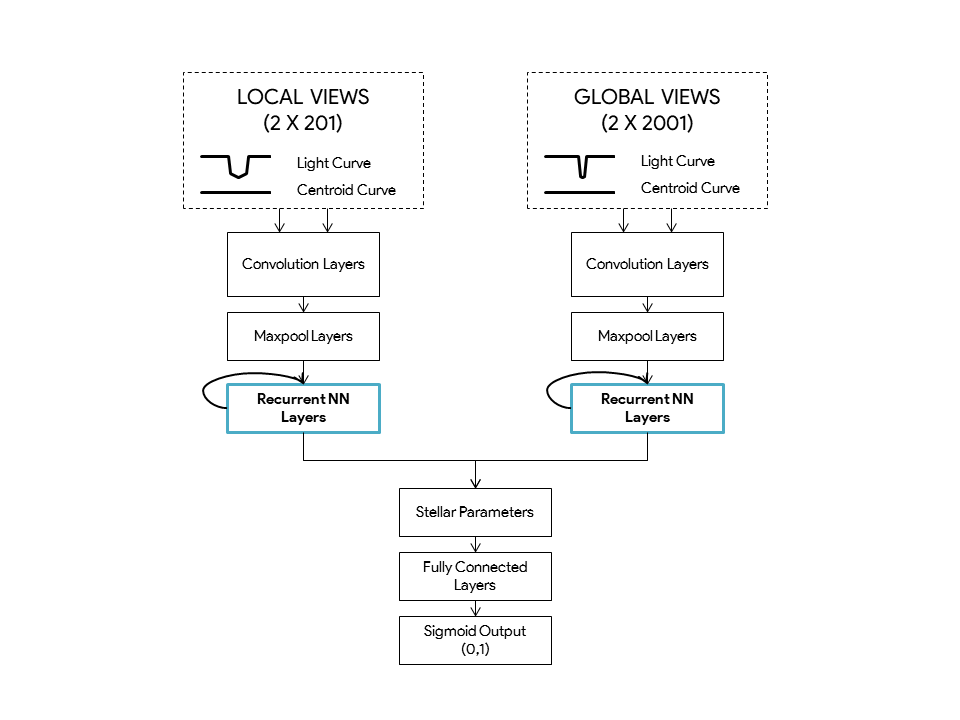
\includegraphics[scale=0.5]{Images/RNN_Model.png}
    \caption{ExoRnet: A proposed high-level model architecture for Classification of Exoplanet Candidates from the TCEs}
    \label{fig:Ansdell}
\end{figure}

We will be considering Exonet as our baseline comparison model as it presents the state-of-the-art results. The main part of our research focuses on vetting of exoplanet candidates. However, we also plan to extend the research to survey the following:
\begin{itemize}
    \item Compare RNN's accuracy for transit detection. The current state-of-art-models use 1D-CNNs (\textbf{Zucker & Giryes}, 2018), phase folding using periodicity ( \textbf{Pearson et al.}, 2018) and 2D-CNNs with phase folding (\textbf{Chintarungruangchai et al.}, 2019)
    \item Classification of non planetary transits into specific classes such as Eclipsing Binaries or Stellar Spots
    \item Preliminay parameterization of detected exo-planets, such as finding the planet radius, by accurately modelling transit depth using a Deep Learning technique
\end{itemize}

\subsection{Data Required}
We plan to use the Kepler Q1-Q17 Data Release 24 light curves from Mikulski Archive for Space Telescopes (MAST) produced by Kepler \textbf{Science Processing Pipeline}. We also plan on using Data Release 30 light curves from TESS, available on MAST. The data will be used in the propotions 8:1:1, meaning, 80\% of the data will be used for Training, 10\% for validation which will be used for hyperparameter tuning and the rest 10\% for testing. 
\subsection{Resources Required}
As data from space based telescopes required for transit classifications is available on NASA Archive and Mikulski Archive for Space Telescopes, we do not have any other specific data requirements. We need computation power for training the system effectively. However, as presented by Shallue and Venderburg (2018), their best model needed 90 minutes to train completely, we extrapolate that the time required to train our models will be almost double of this, due to involvement of recurrent networks. The timeline for classification of transits as planet or non planet candidates can be done in the phases- Data pre-processing, replicating the Exonet architecture for baseline run, researching RNN's effectiveness in the model as a cascaded module, experimenting with several configurations and comparison and surveying of results. The modules require a time commitment of approximately 12 weeks.